%%%%%%%%%%%%%%%%%%%%%%%%%%%%%%%%%%%%%%%%%%%%%%%%%%%%%%%%%%%%%%%%%%%%
% Authors: A. Herrera-Poyatos, F. Herrera
% Tittle: Algoritmo memético equilibrado con diversificación voraz
% 							 CAEPIA 2015
%%%%%%%%%%%%%%%%%%%%%%%%%%%%%%%%%%%%%%%%%%%%%%%%%%%%%%%%%%%%%%%%%%%%

\section{Map Reduce}

	\subsection*{¿Qué es Map Reduce?}

		\begin{frame}{¿Por qué surge Map Reduce?}
	
			\begin{columns}
				\column{0.5\textwidth}
					{\centering\large\color{TurkishRose}\textbf{Problemas de la programación distribuida}}
					\begin{itemize}
						\item Implementaciones a bajo nivel: OpenMP, MPI ...
						\item Reimplementación del mismo tipo de paralelización
						\item Tolerancia a fallos
					\end{itemize}
				\column{0.5\textwidth}
				
					
\includegraphics[width=\textwidth]{./Images/google.png}
			\end{columns}		
			
	
		\end{frame}


		\begin{frame}{¿Cómo funciona map reduce?}
			
			\fontsize{7}{8}\selectfont	
			\centering
			
			\noindent\makebox[\linewidth]{\rule{\textwidth}{0.4pt}}			
			\textbf{Algoritmo:} Obtención del número de ocurrencias de cada una de las palabras de un texto.
			\noindent\makebox[\linewidth]{\rule{\textwidth}{0.4pt}}

			\kern2mm					
			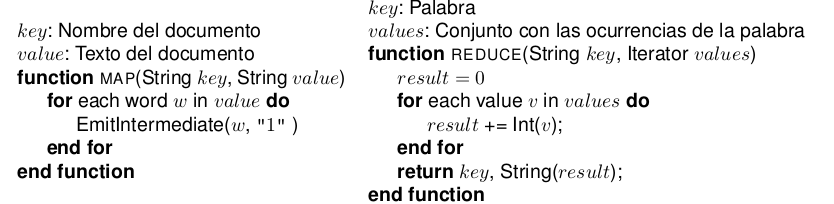
\includegraphics[width=0.88\textwidth]{./Images/count-words.png}		


			\noindent\makebox[\linewidth]{\rule{\textwidth}{0.4pt}}

			\kern2mm					
			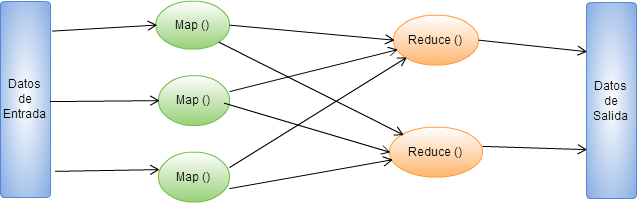
\includegraphics[width=0.9\textwidth]{./Images/MapReduce.png}
		\end{frame}


		\begin{frame}{¿Cómo funciona map reduce?}
			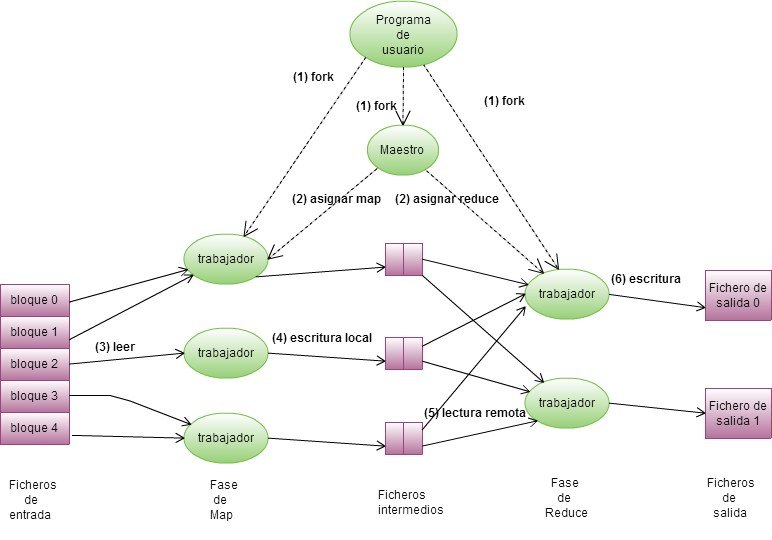
\includegraphics[width=0.9\textwidth]{./Images/MapReduce-MasterWorkers.png}
		\end{frame}

	\subsection*{Software libre}
	
		\begin{frame}{Hadoop}
			
			
		\end{frame}
